\iffalse

Nico Casale
Cody Orazymbetov

ECE 592 Project 1

\fi

\documentclass[]{../ncmathy}

\begin{document}
	
	To develop an implementation of \textit{k-means} in MATLAB, we referenced Wikipedia's \href{https://en.wikipedia.org/wiki/K-means_clustering#Standard_algorithm}{article on K-means}.
	\\\\
	The \textit{k-means} algorithm (\textit{a.k.a.} Lloyd's algorithm) has three main steps:
	
	\begin{enumerate}
	\item Initialize the $k$ centroids, or cluster locations.
	\item Assign each sample of the data to one of the centroids. The centroid with the smallest squared Euclidian distance to the sample is chosen. 
	\item Update each cluster as the centroid (geometric average in $P^2$-Dimensional space, where P is the patch dimension) of the samples that were assigned to it in step 2.
	\item repeat steps 2 and 3 until the assignments no longer change. 
	\end{enumerate}
	
	Note that \textit{k-means} is not guaranteed to find the global optimum clustering, as it is highly dependent on step 1. The initialization is the primary factor in the convergence and quality of the clustering operation. Some notes on initialization are in the next section.
	\\\\
	Below is an example of the output of our \textit{k-means} function on a $[400\times 400]$ image with a patch size of $[2\times 2]$ and 16 clusters. 
	
	\begin{figure}[H]
	\centering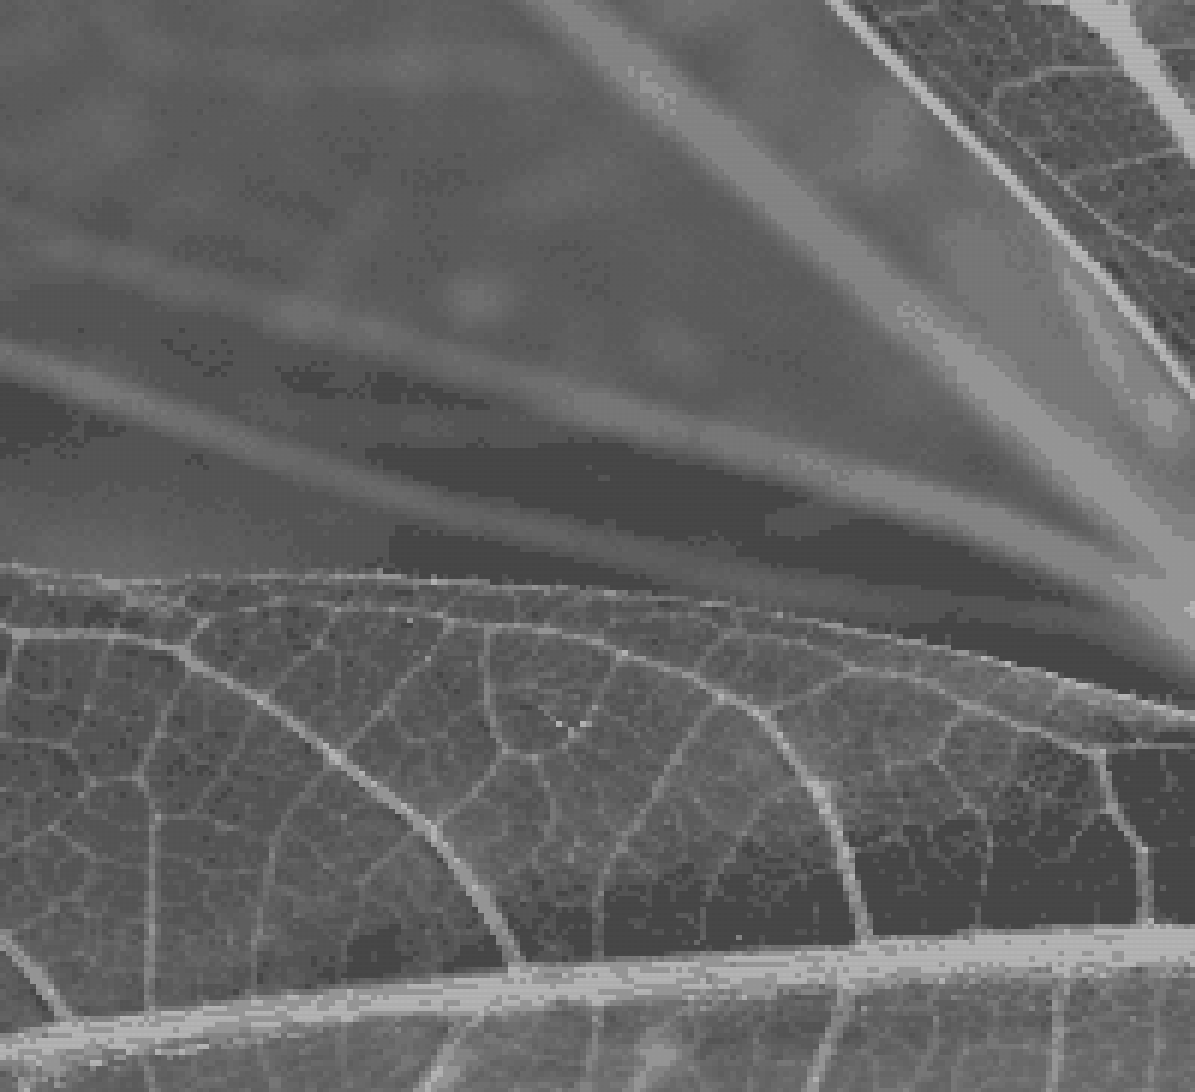
\includegraphics[width=0.6\textwidth]{altkmeans_reconstructed}
	\caption{Example output of \code{kmeans\_alt(.)}.}
	\end{figure}
	
	\subsection{Initialization of \textit{k-means}}
		At first, we took the following approach to initialize the clusters:
			\begin{enumerate}
			\item Find the global minimum and maximum of the pixels in the image.
			\item Generate K linearly spaced points in $\mathbb{R}^{1\times P}$.
			\end{enumerate}
		However, this approach took $\sim$50 iterations to converge. Likewise, because it didn't take into account the statistical distribution of the pixels in the image, it couldn't capture the subtleties of the image where most of its pixels lay. 
		\\\\
		After looking at the Wikipedia page for \textit{k-means}, we noticed that there was some discussion on initialization methods. As a second approach, we tried the Forgy Method, which takes k random samples from the image and uses them as the initial clusters. This method was much more effective as it reduced the number of iterations needed to converge to $\sim$15. As this method is inherently stochastic, some assays would take longer to converge as they were initialized to locations that were distant from the more stable regions. We describe good locations for clusters as `stable regions' because there are an infinite number of clusters and locations that could converge under Lloyd's algorithm. 
	
	\subsection{Timing and Distortion Comparisons}
			The table below illustrates some comparisons between MATLAB's built in \textit{k-means} function and the one we coded. All values were averaged over 20 iterations in MATLAB R2016b. The computer used was a Dell laptop with an Intel Core i3 processor. 
			
			\begin{table}[H]
			\centering\makegapedcells
			\begin{tabular}{||c c c||}
			\hline
			 & MATLAB & Our Implementation \\
			\hline\hline
			Average time & 0.863 & 2.578 \\
			Minimum time & 0.421 & 0.965 \\
			Distortion & 27.386 & 56.191 \\
			\hline
			\end{tabular}
			\caption{Comparison of MATLAB's \textit{k-means} and ours.}\end{table}
			
			Note that our function is both slower and less accurate than MATLAB's by a factor of $\sim$2. In the future, improvements could be made to the initialization procedure to try to get a more accurate representation that takes less time to compute. From a purely computational perspective, the \textit{k-means} exhibits a great deal of parallelism. The result of step 3 is strictly dependent on step 2, but each is parallelizable on its own. In the next section, some details on a potential parallelization of \textit{k-means} are discussed.
	
	\subsection{Profiler Results}
		In analyzing the bottlenecks of the code we wrote to implement \textit{k-means}, we noticed that there is one computationally expensive part of the calculation that is hard to improve outside of parallelization. The figures below illustrate the most time-consuming lines of our function. Note that this screenshot is from a run of our alternate \textit{k-means} function that converged in 9 iterations, a relative minimum given our current implementation.
		
		\begin{figure}[H]
		\centering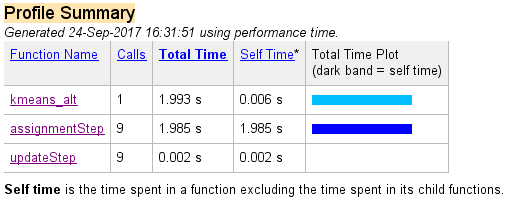
\includegraphics[width=0.65\textwidth]{profiler-top}
		\caption{First page of MATLAB's profiler results.}
		\end{figure}

		\begin{figure}[H]
		\centering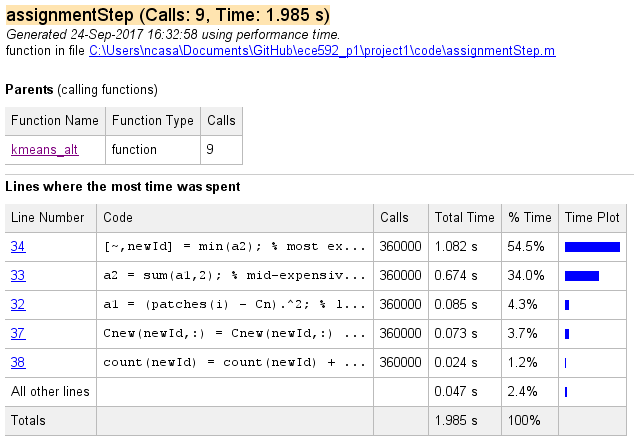
\includegraphics[width=0.7\textwidth]{profiler-assignmentStep}
		\caption{Analysis of the \code{assignmentStep(.)} function.}
		\end{figure}
		
		As shown in the figure, our two most expensive lines deal with the assignment of samples to clusters. In order to determine which of the current clusters a sample belongs to, the code takes the squared Euclidian distance of each point to each of the clusters. The cluster that is closest to the point is assigned. This step is computationally expensive because the function \code{assignmentStep(.)} must sum along the y dimension the distances between each of the pixel values in the patch and the centroids. Then, the \code{min(.)} function has to find the smallest point in the $[K\times 1]$ array. These calls are necessary for quick convergence but negatively impact the time it takes to reach convergence. We tried to use ersatz methods, such as taking the absolute value of the distances instead of squaring them, or taking only the $1^{st}$ column of distances, but these approaches led to less accurate assignment. Even though they were less computationally expensive individually, they led to a higher number of iterations, which totally counteracted the positive effects of the individual computation. 
		\\\\
		If we were to implement \textit{k-means} on a GPU, we could parallelize the thousands of calls to \code{assignmentStep(.)} so that the function would run faster. That, paired with a more effective initialization, would create a good implementation of \textit{k-means} that could be on par with MATLAB.

\end{document}